%
\documentclass[5p,twocolumn,english]{elsarticle}

\usepackage{epstopdf}
\usepackage[caption=false]{subfig}
\usepackage{hyperref}

\usepackage{amsmath,amssymb,amsfonts}
%\usepackage{algorithmic}
\usepackage{graphicx}
\usepackage{framed,multirow}
\usepackage{gensymb}
\usepackage{textcomp}

\usepackage{supertabular}

\usepackage{multirow}
\usepackage{color,colortbl}
\usepackage{float}
\usepackage{setspace}
%\usepackage[justification=justified]{caption}
%%\usepackage[justification=centering]{caption}

%\usepackage{soul}

\DeclareRobustCommand{\hlight}[1]{{\sethlcolor{yellow}\hl{#1}}}

\begin{document}
%
% paper title
\begin{frontmatter}

\title{Vision based open-space parking management system using YOLOv10}

\author[first]{Bermal Arato\~glu}%%% First author
\ead{bermal.aratoglu@ogr.sakarya.edu.tr}

\author[first]{Bu\~gra \c{C}elebi}%%% Second author
\ead{bugra.celebi@ogr.sakarya.edu.tr}

\author[first]{Ahmet \"Ozmen\corref{cor}}%%% Third author
\ead{ozmen@sakarya.edu.tr} 

\cortext[cor]{Corresponding Author: A. \"Ozmen, Tel: +90(264)295 6984, Fax: +90(264)295 6978}

\address[first]{Department of Software Engineering, Sakarya University, Sakarya, 54050, TURKEY}%%% Author address here

%% Abstract
%%
\begin{abstract}

%% What is new? What is the obtained results (achieved)
Efficient parking management has become a critical challenge in modern urban environments and large facilities, such as shopping malls, university campuses, and public spaces. Due to physical insufficiency and the inefficient use of parking lots, the significant increase in demand for parking spaces cannot be adequately addressed. This growing disparity between supply and demand leads to congestion, driver frustration, and wasted resources. Traditional parking systems, which rely heavily on manual monitoring or sensor based solutions, often struggle to meet the needs of these dynamic and high demand environments. Expensive implementation costs, limited scalability, and susceptibility to environmental factors further exacerbate the challenges of managing parking efficiently in such contexts. Bu makalede yeni olan nedir? YAZILACAK. Bu çalışma sonunda elde edilen başarı nedir YAZILACAK.
\end{abstract}

\begin{keyword}
  Vision based parking monitoring \sep open space management \sep vehicle tracking \sep vehicle counting
\end{keyword}


\end{frontmatter}

%%\maketitle

%%
%%  body.tex
%%---------
%%%%%%%%%%%%%%%%%%%%%%%%%%%%%%%%%%%%%%%%%%%%%%%%%%%%%%%%%%%%%%%%%%%%%

\section{Introduction}
\label{sec_intro}

%% Giris, motivation
Efficient parking management has become a critical challenge in modern urban environments and large facilities, such as shopping malls, university campuses, and public spaces.

% Why do we need open park management and vision based system? 
Traditional parking space management systems focus on monitoring vehicle movement using various tools. While these systems generally provide a basic overview of parking lot occupancy, they suffer from significant limitations, particularly in terms of scalability and reliability. Moreover, traditional systems are prone to maintenance issues and hardware failures, leading to periods of downtime where data collection becomes inconsistent or inaccurate. This unreliability creates gaps in the data, preventing parking lot administrators from gaining actionable insights or optimizing operations effectively. In short, there is a pressing need for a robust, efficient system capable of continuously collecting and processing data for parking space management, ensuring real-time insights and operational reliability under diverse conditions. 

% Existing approaches
  


  

% Brief about proposed approach


% Fig 1
\begin{figure}[t]
	\centering
	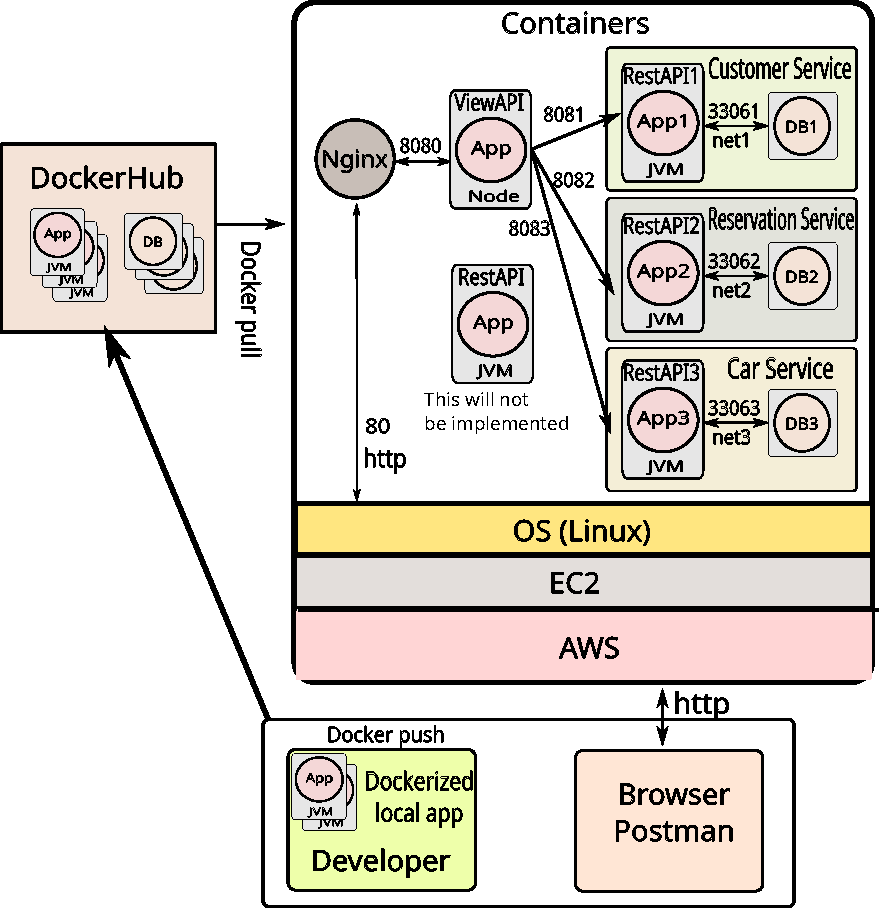
\includegraphics[width=0.35\textwidth]{figs/fig1.pdf}
	\caption{Single camera vehicle detection and tracking.}
	\label{fig1}
\end{figure}

This study focus on centralized algorithmic method development for multiple video-stream that comes from cheap multiple cameras simultaneously. The proposed system can be used in an integrated management system that combines real-time vehicle tracking, speed analysis, and entry/exit counting. Hence, the research aim is to extend the view in one axis region without requiring expensive hardware for video stream processing. We introduce a "virtual context" concept which refers to a single large frame which is formed by combining synchronized and normalized video frames coming from separate cameras. In this solution, detector and tracker algorithm input will be one large frame, where complex object/vehicle fusion tasks are not necessary as studied in some other work \cite{land11060886}.

In this study, the frames are normalized and synchronized to form a single meaningful virtual context based on the multi-camera setup. The problematic situations and proposed solutions are listed as follows:
\begin{itemize}
	\item Overlapping frames:
	\item Non-overlapping frames:
	\item Cameras are not aligned in an axis:
	\item Cameras are not identical:
	\item Different angle situations:
\end{itemize}  

%% Paper organization
A brief outline of remaining parts of the paper is as follows: In Section~\ref{sec_related}, a summary of related literature on multi camera-based vehicle detection and tracking methods is presented.  In Section~\ref{sec_method}, the proposed approach, data structures and computation flow are presented in details.  In Section~\ref{sec_results} experimental results, comments and discussions about the results are presented.

\section{Related work}
\label{sec_related}

% Giris
Cameras are cheap and valuable information resource for traffic observation. However, processing video streams that comes multiple cameras creates a challenging work due to 1) required processing power increases, 2) objects detected on different views challenging problem to evaluate in on context.



A few group worked on different setup for multi-camera setup in literature \cite{olagoke}. In some studies objects detected from individual streams and then these objects are fused in one context for tracking. At another approach, detection and tracking are done over individual streams and associated the objects afterwards as shown in \ref{fig2}.

% Fig 2
\begin{figure}[t]
	\centering
%	\includegraphics[width=0.45\textwidth]{figs/pdf/intersection_multi.pdf}
	\caption{Use of multi-camera setup and fusion of objects found on different contexts for vehicle detection and tracking.}
	\label{fig2}
\end{figure}

\subsection{Multi camera systems}

% Position of cameras 
A wider view can be obtained by using multiple cameras which eventually increases the accuracy of vision-based monitoring systems. 
 
Problem: How to follow objects that pass through individual views coming from different cameras?

{\bf Studies in the area and proposed solutions in the literature:}

Solution 1: Cooperative multi-camera system proposed for traffic surveillance system \cite{YANG}. Need more explanation.  

Solution 2: Another study proposes highway trajectory refinement method \cite{zhang}.

Solution 3: Need to do a bit more research on the issue and find out what people have done.


\subsection{Object Detection using YOLO}

Object detection from video streams has recently become a simple task by the invention of complex deep learning algorithms such as YOLO. However, the problem arises when multiple camera is needed to monitor a larger areas.

\subsection{Vehicle tracking on multi-camera systems}

Tracking objects from video streams is a challenging task due to complexity of the algorithms and required computational power.

\section{Proposed method}
\label{sec_method}

1) Extending planar view: This is a 2D frame enlargement study. N camera are shooting same target with a displacement in the same axis to extend the visibility.

Problems: a) Finding overlapping sections. b) Heterogeneous cameras may become problem since video formats may change. c) Position of the cameras, and vehicle distances.

Figure \ref{fig3} shows the proposed approach which is a novel solution to aforementioned problems, such as it requires less compute power, and merging the streaming frames to create a virtual context is a less complex task comparing to object fusion.

% Fig 3
\begin{figure}[t]
	\centering
%	\includegraphics[width=0.45\textwidth]{figs/pdf/merge.pdf}
	\caption{Use of multi-camera setup to extend the visible target for vehicle detection and tracking.}
	\label{fig3}
\end{figure}


The following situations must be studied see Figure \ref{situations}:
1) Perfectly aligned camera setup: In this case only merging process for video frames is performed.
2) Cameras are in the same axis, however, there are missing parts in the shooting region: Extra effort is necessary to fix tracking, such as Kalman filter.
3) Overlapping shooting in the same axis: A pre-processing for overlapped frame sections removal required.
4) Unaligned cameras: Transformation is required over the frames to make object sizes equal.

% Fig 4
%\begin{figure*}[t]
%	\centering
%	\subfloat[][]{
%	\includegraphics[width=0.18\textwidth]{figs/pdf/conf1.pdf}}	
%	\subfloat[][]{
% \hspace{2cm}\includegraphics[width=0.28\textwidth]{figs/pdf/conf2.pdf}} \\
%	\subfloat[][]{
%	\includegraphics[width=0.18\textwidth]{figs/pdf/conf3.pdf}}
%	\subfloat[][]{
%	\hspace{2cm}\includegraphics[width=0.26\textwidth]{figs/pdf/conf4.pdf}}
%	\caption{a) Perfectly aligned camera setup. b) Non-covering video shooting. c) Overlapping shooting. d) Unaligned camera setting.}
%	\label{aligned}
%\end{figure*} 


%2) Extending planar view with an angle (2 camera study):
%
%Problems: How to convert (transfer) and then process the video data? Vehicle detection becomes a challenging task since more cameras may see the same object from different perspectives.
%
%3) Cylindrical context:  
%
%Problem: This is a bit more challenging comparing to the previous work. A cylindrical context can be created by means of transformations. However, how to apply object detection approaches to this cylindrical context? Very challenging. We are going to search a solution to this problem. Once we solve it -- Bingo!


\section{Experimental setup}

We need to explain data set that we used to measure performance of proposed approach and then compare it with existing work.


\section{Results and discussion}
\label{sec_results}

%% General comments
Accurate vehicle trajectory extraction provides more precise ``high-level traffic flow information'', but this fully depends on the low-level traffic data such as vehicle detection and tracking information.  In turn, vision-based vehicle detection and tracking systems mostly rely on modern data processing methods such as deep or machine learning algorithms. The input video data must be clear to get a successful output from the image processing systems. 


\section{Conclusion}

In this study, a new concept "virtual context" introduced for multi-camera based monitoring systems. The proposed solution increases the accuracy of such systems while decreasing the  required computing power for video processing.


\bibliographystyle{ieeetr}
\bibliography{open_park}
\end{document}


